\documentclass[12pt]{article}
\usepackage[left=2cm, right=2cm, top=2cm]{geometry}
\usepackage[utf8]{inputenc} 
\usepackage{mdframed} %For framing the title
\usepackage{graphicx} % to include images
\usepackage{amsmath} % For math mode
\usepackage{mathtools} %for bmatrix*
\usepackage{caption} % For captions
\usepackage{subcaption} % To use caption while using mini page
\usepackage{amssymb} % To use math symbols
\usepackage{multirow} %To combine multiple rows in a table
\usepackage[table]{xcolor} %To color rows / columns in table
\usepackage{titling} %To vertically center the title page
\usepackage{hyperref} %for URL
\usepackage{float} %For [H] in includegraphics
\usepackage[section]{placeins} %Prevents floats before a section
\usepackage{textcomp} %For degree symbol
\usepackage{enumerate} %For roman numbers
\usepackage{enumitem} %for reference numbers
\usepackage{titling} %For the centering of title page
\usepackage{url} %for URL linebreak
\usepackage{breakurl} % for URL line break
\PassOptionsToPackage{hyphens}{url}\usepackage{hyperref} % for URL line break
\usepackage{exsheets} %For itemize in a line
\usepackage{tasks} %For itemize in a line
%\usepackage[inline]{enumitem}    %For itemize in a line

%----------------------------PYTHON TEMPLATE -------------------------------------
\usepackage{listings}
\usepackage{color} %red, green, blue, yellow, cyan, magenta, black, white
\usepackage{setspace}
\definecolor{Code}{rgb}{0,0,0}
\definecolor{Decorators}{rgb}{0.5,0.5,0.5}
\definecolor{Numbers}{rgb}{0.5,0,0}
\definecolor{MatchingBrackets}{rgb}{0.25,0.5,0.5}
\definecolor{Keywords}{rgb}{0,0,1}
\definecolor{self}{rgb}{0,0,0}
\definecolor{Strings}{rgb}{0,0.63,0}
\definecolor{Comments}{rgb}{0,0.63,1}
\definecolor{Backquotes}{rgb}{0,0,0}
\definecolor{Classname}{rgb}{0,0,0}
\definecolor{FunctionName}{rgb}{0,0,0}
\definecolor{Operators}{rgb}{0,0,0}
\definecolor{Background}{rgb}{0.98,0.98,0.98}
\lstdefinelanguage{Python}{
numbers=left,
numberstyle=\footnotesize,
numbersep=1em,
xleftmargin=1em,
framextopmargin=2em,
framexbottommargin=2em,
showspaces=false,
showtabs=false,
showstringspaces=false,
frame=l,
tabsize=4,
% Basic
basicstyle=\ttfamily\small\setstretch{1},
backgroundcolor=\color{Background},
% Comments
commentstyle=\color{Comments}\slshape,
% Strings
stringstyle=\color{Strings},
morecomment=[s][\color{Strings}]{"""}{"""},
morecomment=[s][\color{Strings}]{'''}{'''},
% keywords
morekeywords={import,from,class,def,for,while,if,is,in,elif,else,not,and,or,print,break,continue,return,True,False,None,access,as,,del,except,exec,finally,global,import,lambda,pass,print,raise,try,assert},
keywordstyle={\color{Keywords}\bfseries},
% additional keywords
morekeywords={[2]@invariant,pylab,numpy,np,scipy},
keywordstyle={[2]\color{Decorators}\slshape},
emph={self},
emphstyle={\color{self}\slshape},
%
}
\linespread{1.3}
%-----------------------------------------------------------------------------------------

%Centering of title page
\renewcommand\maketitlehooka{\null\mbox{}\vfill}
\renewcommand\maketitlehookd{\vfill\null}

%\begin{titlepage}
\title{\bf CPSC 8810 - Deep Learning\\
Deep Learning Model to Detect CyberBully Actions in Images}
\author{Submitted By:\\	Vivek Koodli Udupa - (C12768888) \\
		Shashi Shivaraju - (C88650674)\\}
\date{Clemson University \\\today}
%\end{titlepage}


%%To make the title page center vertically centered
%\renewcommand\maketitlehooka{\null\mbox{}\vfill}
%\renewcommand\maketitlehookd{\vfill\null}

\begin{document}
\sloppy %to remove line breaks
%\begin{mdframed}
%Displaying Title
\begin{titlingpage}
\maketitle
\pagenumbering{gobble}% Remove page numbers (and reset to 1)
\end{titlingpage}
%\end{mdframed}\begin{document}


\pagenumbering{roman} %set page numbering to roman

%----------------------------------------------------------------------------------------
%	REPORT ABSTRACT
%----------------------------------------------------------------------------------------
\newpage
\begin{abstract}
\thispagestyle{plain}
\addcontentsline{toc}{section}{\bf Abstract}
This report explains the process involved in  a Convolutional Neural Network to detect and classify various cyberbully actions in an image. 
\end{abstract}
\newpage

\pagenumbering{arabic} %set page numbering to arabic
%----------------------------------------------------------------------------------------
%	Introduction
%----------------------------------------------------------------------------------------
% Introduction Chapter
\section{Introduction}
This report considers the problem of detection and calssification of cyberbully actions caputired in an image using Deep learning models.  \\

Cyberbullying is bullying that takes place over digital devices like cell phones, computers, and tablets. Cyberbullying can occur through SMS, Text, and apps, or online in social media, forums, or gaming where people can view, participate in, or share content. Cyberbullying includes sending, posting, or sharing negative, harmful, false, or mean content about someone else. Some cyberbullying crosses the line into unlawful or criminal behavior. With the prevalence of social media and digital forums, comments, photos, posts, and content shared by individuals can often be viewed by strangers as well as acquaintances. The content an individual shares online – both their personal content as well as any negative, mean, or hurtful content – creates a kind of permanent public record of their views, activities, and behavior. This public record can be thought of as an online reputation, which may be accessible to schools, employers, colleges, clubs, and others who may be researching an individual now or in the future. Cyberbullying can harm the online reputations of everyone involved – not just the person being bullied, but those doing the bullying or participating in it.[1] \\ 

Deep learning is a subset of machine learning where artificial neural networks, algorithms inspired by the human brain, learn from large amounts of data. The term  ‘deep learning’ because the neural networks have various (deep) layers that enable learning. Deep learning allows machines to solve complex problems even when using a data set that is very diverse, unstructured and inter-connected. The more deep learning algorithms learn, the better they perform. [2] \\

This report describes modeling of a deep learning network based on the concept of convolutional neural network for detecting and classifying cyberbully actions for a given image. The cyberbullying actions considered in this project are laughing, pulling-hair, quarrel, slapping, punching, stabbing, gossiping, strangle and isolation. The designed model is trained using the provided image dataset which contain above mentioned 9 categories of cyberbully actions in them.   

\newpage

\section{Methods}
In deep learning, a convolutional neural network (CNN, or ConvNet) is a class of deep neural networks, most commonly applied to analyzing visual imagery.[3] A convolutional neural network consists of an input and an output layer, as well as multiple hidden layers. The hidden layers of a CNN typically consist of convolutional layers, ReLU layer i.e. activation function, pooling layers, fully connected layers and normalization layers.[4] \\ 

Convolutional networks were inspired by biological processes in that the connectivity pattern between neurons resembles the organization of the animal visual cortex. CNNs use relatively little pre-processing compared to other image classification algorithms. This means that the network learns the filters that in traditional algorithms were hand-engineered. This independence from prior knowledge and human effort in feature design is a major advantage. \\

The implementation of our model based on CNN using an open source machine learning library PyTorch is described in the section below. 

\subsection{Implementation of CNN Model}
\label{sec:model_def}
Our model is implemented using the following layers: 
\begin{enumerate}
	\item {\textbf{Convolutional Layer:}} The convolutional layer is the core building block of a CNN. The layer's parameters consist of a set of learnable filters (or kernels). During the forward pass, each filter is convolved across the width and height of the input volume, computing the dot product between the entries of the filter and the input and producing a 2-dimensional activation map of that filter. As a result, the network learns filters that activate when it detects some specific type of feature at some spatial position in the input.
	
	\item {\textbf{ReLU layer:}} ReLU is the abbreviation of rectified linear unit, which applies the non-saturating activation function 
\begin{equation}	
	f(x)=max(0, x)
\end{equation} It effectively removes negative values from an activation map by setting them to zero. It increases the nonlinear properties of the decision function and of the overall network without affecting the receptive fields of the convolution layer. 

	\item {\textbf{Max Pooling:}} Another important concept of CNNs is pooling, which is a form of non-linear down-sampling. Max pooling is the most common non-linear function for down-sampling. It partitions the input image into a set of non-overlapping rectangles and, for each such sub-region, outputs the maximum. 
	
	\item \textbf{Fully Connected Layer:} Finally, after several convolutional and max pooling layers, the high-level reasoning in the neural network is done via fully connected layers. Neurons in a fully connected layer have connections to all activations in the previous layer, as seen in regular (non-convolutional) artificial neural networks. Their activations can thus be computed as an affine transformation, with matrix multiplication followed by a bias offset. 
	
	\item \textbf{Dropout Layer:} A single model can be used to simulate having a large number of different network architectures by randomly dropping out nodes during training. This is called dropout and offers a very computationally cheap and remarkably effective regularization method to reduce over fitting and generalization error in deep neural networks.[5]

\end{enumerate}

The implementation details of our model is as follows: 
\begin{enumerate}
	\item \textbf{Image Pre-Processing: } The given input image is converted into mono-channeled, gray scale image of size 256 x 256. Then it is converted to a PyTorch tensor image and its values are normalized with a mean of 0.5 and Standard Deviation of 0.5.   
  
	\item \textbf{Convolution Layer 1:} The input to this layer is a preprocessed tensor image from the previous layer. This layer performs 2D convolution using a 3x3 kernel with stride set to 1 and padding enabled to produce an output which is a 16 channel feature map. 
	
	\item \textbf{ReLU Layer 1:} This layer applies a relu activation function to the 16 channel feature map.
	 
	 \item \textbf{Max Pooling Layer 1:} This layer down-samples the 256 x 256 16 channel feature map to 128 x 128 16 channel feature map.
	 
	 \item \textbf{Convolution Layer 2:} The input to this layer is the 16 channel 128 x 128 feature map from the previous layer. This layer performs 2D convolution using a 3 x 3 kernel with stride set to 1 and padding enabled to produce an output which is a 32 channel feature map. 
	 
	 \item \textbf{ReLU Layer 2:} This layer applies a relu activation function to the 32 channel feature map.
	 
	 \item \textbf{Max Pooling Layer 2:} This layer down-samples the 128 x 128 32 channel feature map to 64 x 64 32 channel feature map.
	 
	 \item \textbf{Flattening Layer: } This layer flattens the 2D feature map to 1D feature map. 
	 
	 \item \textbf{Dropout Layer:} This layer randomly zeros some of the element of the input tensor with probability 0.4. 
	 
	 \item \textbf{Fully Connected Layer 1:} This layer maps the feature map into 100 neurons.
	 
	 \item \textbf{ReLU Layer 3:} This layer applies a relu activation function to the output of Fully Connected Layer 1.
	 
	 \item \textbf{Fully Connected Layer 2:} This layer maps 100 neurons into 10 categories of classification.
	 
\end{enumerate}

\subsection{Training the CNN Model}
\label{model_train}
To train a deep learning model, the following parameters are considered:
\begin{enumerate}
	\item \textbf{Epoch:} An epoch describes the number of times the algorithm sees the entire data set. So, each time the algorithm has seen all samples in the dataset, an epoch has completed.
	\item \textbf{Batch Size:} The total number of training examples present in a single batch, wherein a batch is a subset of the entire data set. 
	\item \textbf{Iteration:} The number of batches needed to complete one Epoch.
	\item \textbf{Learning Rate:} The learning rate or step size in machine learning is hyper-parameter which determines to what extent newly acquired information overrides old information.	
\end{enumerate}

The implemented model is trained using the below mentioned configuration:
\begin{enumerate}
	\item Epoch = 25	
	\item Batch Size = 1
	\item Learning Rate = 0.0001
\end{enumerate}

The model is trained with the given training dataset as per the below mentioned algorithm:
\begin{enumerate}
	\item Initialize the CNN model with default parameters. 
	\item Create an instance of Adam optimizer for setting the learning rate
	\item Create an instance of cross entropy loss
	\item Initialize the optimizer with zero gradients \label{grad_clear}
	\item Feed a training input image from the current batch to the model to perform forward propagation
	\item After the completion of forward propagation, calculate the cross entropy loss
	\item Perform back propagation to minimize the loss
	\item Update gradients
	\item Iterate through step \ref{grad_clear} for all the batches in the training dataset
	\item Repeat the above steps for the given number of epochs
	\item Save the trained model for testing purpose
	
\end{enumerate}


Please refer the appendix for the python implementation of the above described model. 
\newpage

\section{Results}
The network described in section \ref{sec:model_def} was trained using 2494 images split into 10 categories. For a batch size of 1, 15 epochs and a learning rate of 0.0001, the following results were observed. \\

\noindent
The training accuracy(single execution) was found to be 98.08\% . \\

\noindent
The network was tested using the following images. \\

\noindent
The image for the first test is pulled out from the training dataset. Figure \ref{fig:quarrel} belongs to the \lq{quarrel}\rq{} category. The purpose of this test is to check if the network can recognize an image from the training dataset. 
\begin{figure}[H]
\centering
  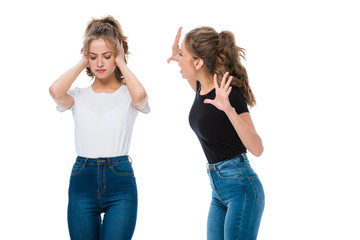
\includegraphics[width=.4\linewidth]{./Images/quarrel.jpg}
  \caption{quarrel}
  \label{fig:quarrel}
\end{figure}
The network classified Figure \ref{fig:quarrel} as \lq{quarrel}\rq{} category. \\

\noindent
The images used for the further tests are images that the network has never seen during the training phase. The purpose of these tests is to check if the network has learned any features based upon which it can categorize images into its respective categories. \\

A Human being would classify Figure \ref{fig:gossip1} as two girls in the foreground gossiping about the third girl in the background. Thus this image falls under the \lq{gossiping}\rq{} category. 
\begin{figure}[H]
\centering
  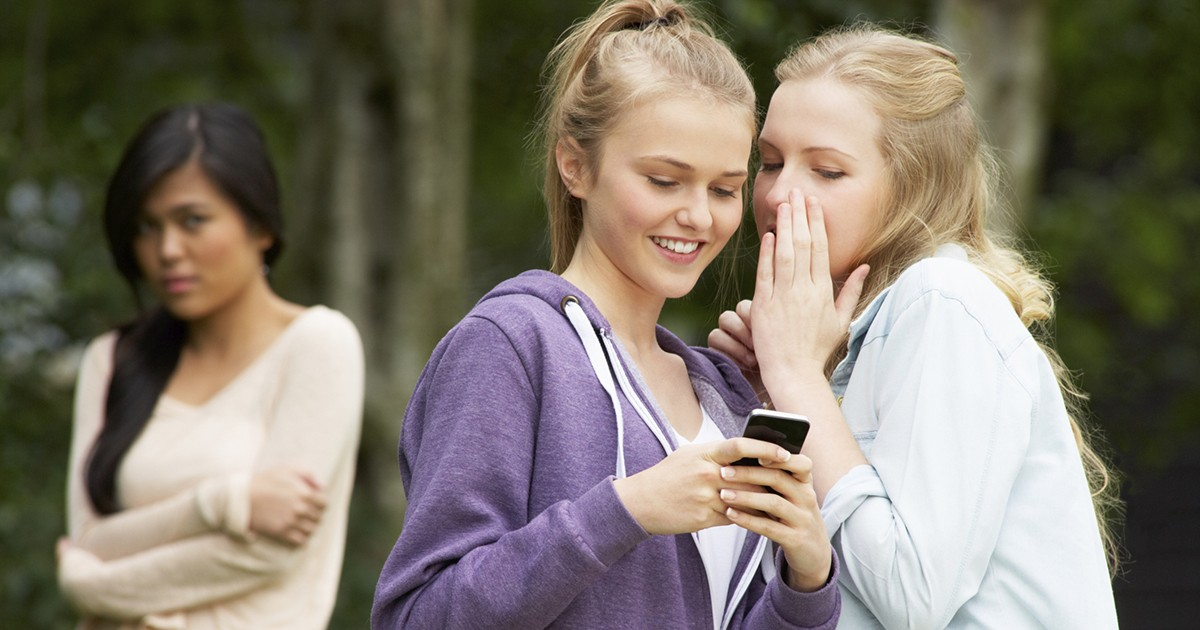
\includegraphics[width=.4\linewidth]{./Images/gossiping1.jpg}
  \caption{gossiping}
  \label{fig:gossip1}
\end{figure}
The network classified Figure \ref{fig:gossip1} to be in the  \lq{strangle}\rq{} category. \\

Upon inspection, Figure \ref{fig:gossip2} appears to comprise of two girls in the background gossiping about the girl in the foreground. Again this is an instance of \lq{gossiping}\rq{}
\begin{figure}[H]
\centering
  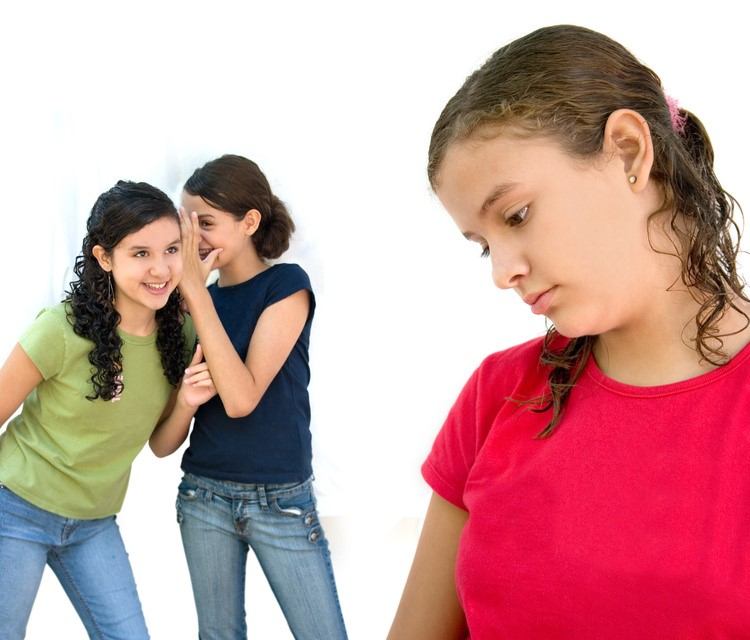
\includegraphics[width=.4\linewidth]{./Images/gossiping2.jpg}
  \caption{Another instance of gossiping}
  \label{fig:gossip2}
\end{figure}
The network classified Figure \ref{fig:gossip2} to be in the \lq{isolation}\rq{} category. \\

Figure \ref{fig:isolation} is quiet straightforward. It represents a girl not being accepted/included in a group of kids. Thus this image falls under the \lq{isolation}\rq{} category. \\
\begin{figure}[H]
\centering
  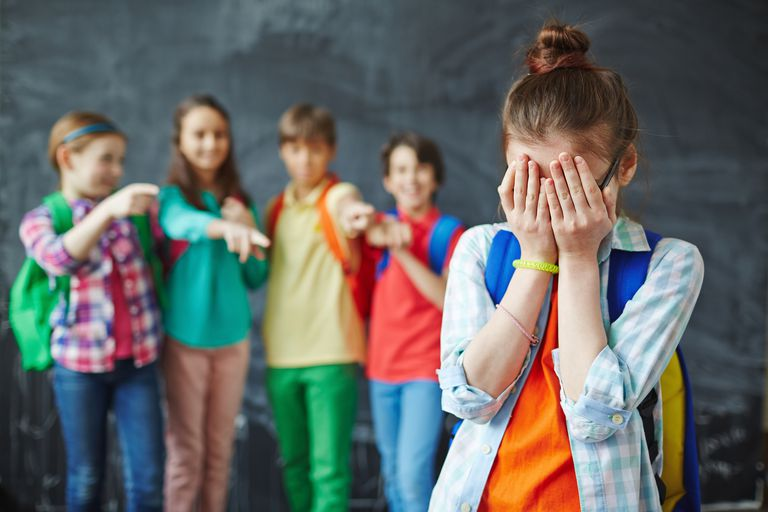
\includegraphics[width=.4\linewidth]{./Images/isolation1.jpg}
  \caption{isolation}
  \label{fig:isolation}
\end{figure}
The network classified Figure \ref{fig:isolation} as \lq{punching}\rq{} category. \\

\newpage

\section{Conclusion}
The goal of this project is to develop a deep neural network that taken an image as input and categorizes it into one of the 10 below mentioned categories.
\begin{enumerate}
	\item Gossiping
	\item Isolation
	\item Laughing
	\item Pulling hair
	\item Punching
	\item Quarrel
	\item Strangle
	\item Slapping
	\item Stabbing
	\item Non bullying
\end{enumerate}
The neural network was developed using PyTorch. The training dataset for the network was made up of 2494 images belonging to the 10 above mentioned categories. The training accuracy for a single run was observed to be 98\%. Four testing examples are mentioned in this report. \\

When the network was presented with an image from the training dataset, it had no problem in predicting the category of the image. The image for this test was taken from the \lq{quarrel}\rq{} category(Figure \ref{fig:quarrel}) and the network predicted it correctly. This confirms that the network actually recognizes the training images and it is not just randomly predicting the image category. \\

For the next three tests, the network was given images that it had never seen before. Here the network is expected to recognize a set of features(in the test image) that it has learnt in the training phase to predict the category of bullying. \\

When the network was tested with Figure \ref{fig:gossip1}, Which is an instance of \lq{gossiping}\rq{} the network wrongly classified it as \lq{strangle}\rq{}. Since the subject in Figure \ref{fig:gossip1} seem to be very close to each other, the network confuses it with \lq{strangling}\rq{}. The reason for this wrong prediction could be that the network has not learnt enough features to clearly distinguish between strangling and gossiping. A deeper network with more complex structure could help the network extract more features. \\

Figure \ref{fig:gossip2} is a complicated image compared to the other test images. This image could either be gossiping or isolation. The girl in the foreground appears to be isolated from the group in the background who are gossiping. The network classified this image to be of the \lq{isolation}\rq{} category. This is probably because the network weighs the foreground subject more than the background. Having a bounding box label would probably help the network prioritize the subject more accurately. \\

Figure \ref{fig:isolation} clearly falls under the \lq{isolation}\rq{} category. But the network classified it as punching. Over-fitting could be the cause for this result. Adding a better dropout layer might refrain the network from over-fitting. \\

In conclusion the model defined in section \ref{sec:model_def} is shallow. Such a basic CNN struggles to deal with images that does not directly fall under a single category of bullying. Having an object detection model such as the YOLO or the RCNN would help in better image classification. Having a pre-trained model like the Resnet or the VGG-16 would improve the test accuracy significantly. The type of image labeling also plays a significant role. Having boundary box labeling might aid the network in more accurate subject prioritization.   


\section{Future Work}
Based on the Results, the following changes are planned to improve the network accuracy. 
\begin{enumerate}
	\item Implement YOLO and RCNN for object detection
	\item Implement a deeper network structure for more feature extraction
	\item Label the images using Boundary box labeling
	\item Incorporate a pre-trained model to improve accuracy
	\item Increase the training image dataset
\end{enumerate}


 
 
\newpage
\section{References}
\begin{enumerate}[label={[\arabic*]}]
\item \url{https://www.stopbullying.gov/cyberbullying/what-is-it/index.html}
\item \url{https://www.forbes.com/sites/bernardmarr/2018/10/01/what-is-deep-learning-ai-a-simple-guide-with-8-practical-examples/#434cffaa8d4b}
\item \url{https://en.wikipedia.org/wiki/Convolutional_neural_network#Convolutional}
\item \url{https://cs231n.github.io/convolutional-networks/}
\item \url{https://machinelearningmastery.com/dropout-for-regularizing-deep-neural-networks/}
\end{enumerate}
\newpage

\section{Appendix}
\subsection{Bully Detection CNN Model}
\lstinputlisting[language=Python]{../detection_Model.py}
\subsection{Training Code}
\lstinputlisting[language=Python]{../training.py}
\subsection{Test Code}
\lstinputlisting[language=Python]{../test.py}


\end{document} 